\subsection{System Integration \& Notification Activity}

\begin{figure}[H]
    \centering
    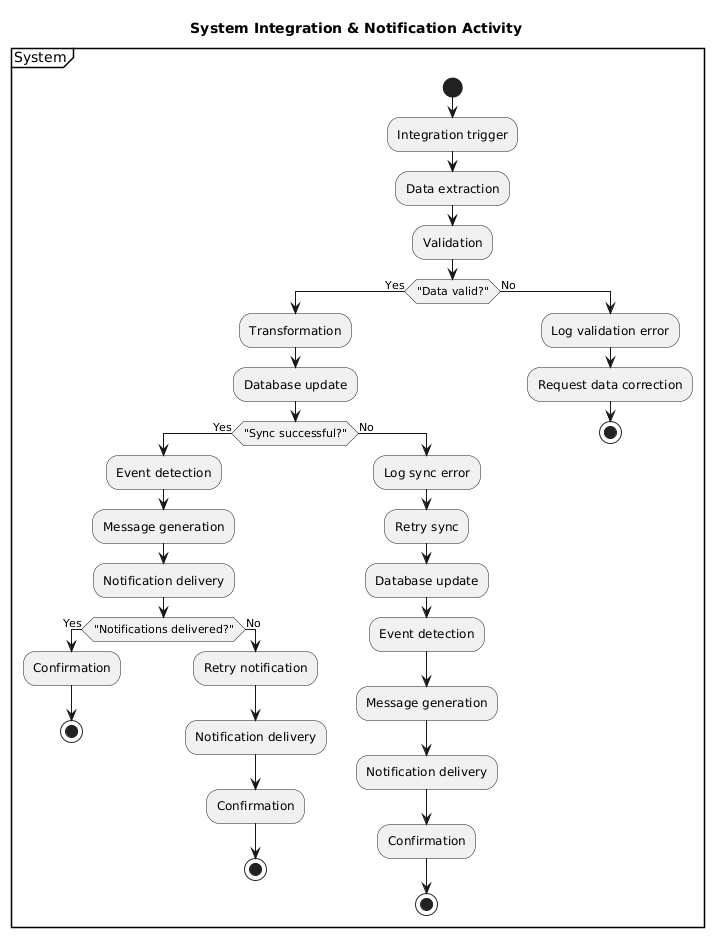
\includegraphics[width=0.9\textwidth]{graphics/chapter4/system/sys_noti.png}
    \caption{System Integration \& Notification Activity}
    \label{fig:Sys_Noti}
\end{figure}

\newpage 

\noindent \textbf{Description}
\begin{enumerate}
  \item \textbf{System}: Integration trigger detected; initiates data extraction from HCMUT systems.
  \item \textbf{System}: Performs data validation to ensure integrity and format compliance.
  \item \textbf{Decision}: Is data valid?
    \begin{enumerate}
        \item \textbf{Yes:} Continue to transformation.
        \item \textbf{No:} Log validation error and request data correction. \emph{Flow ends.}
    \end{enumerate}
  \item \textbf{System}: Transforms data to system format and updates local database.
  \item \textbf{Decision}: Is synchronization successful?
    \begin{enumerate}
        \item \textbf{Yes:} Continue to notification process.
        \item \textbf{No:} Log sync error, retry synchronization, then continue.
    \end{enumerate}
  \item \textbf{System}: Detects notification events and generates appropriate messages.
  \item \textbf{System}: Delivers notifications to relevant users through multiple channels.
  \item \textbf{Decision}: Are notifications successfully delivered?
    \begin{enumerate}
        \item \textbf{Yes:} Send confirmation. \textit{Flow ends.}
        \item \textbf{No:} Retry notification delivery, then send confirmation. \textit{Flow ends.}
    \end{enumerate}
\end{enumerate}